
\chapter{Gráficos do Experimento 4 da Etapa 1}

As Figuras \ref{fig:graphRPM-01}-\ref{fig:graphRPM-10} apresentam a evolução do VPL da melhor solução, da pior solução e a média da população das dez execuções do Algoritmo Genético de Regime Permanente Modificado durante o Experimento 4 da Etapa 1 ($AG^{RPM}$).

\begin{figure}[H]
\centering
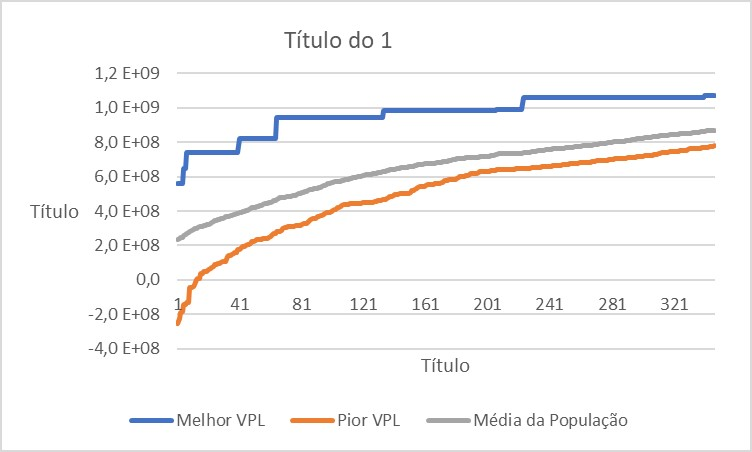
\includegraphics[scale=1]{apxD/1}
\caption{Evolução do VPL para a primeira execução da primeira versão modificada de Algoritmo de Regime Permanente.}
\label{fig:graphRPM-01}
\end{figure}

\begin{figure}[H]
\centering
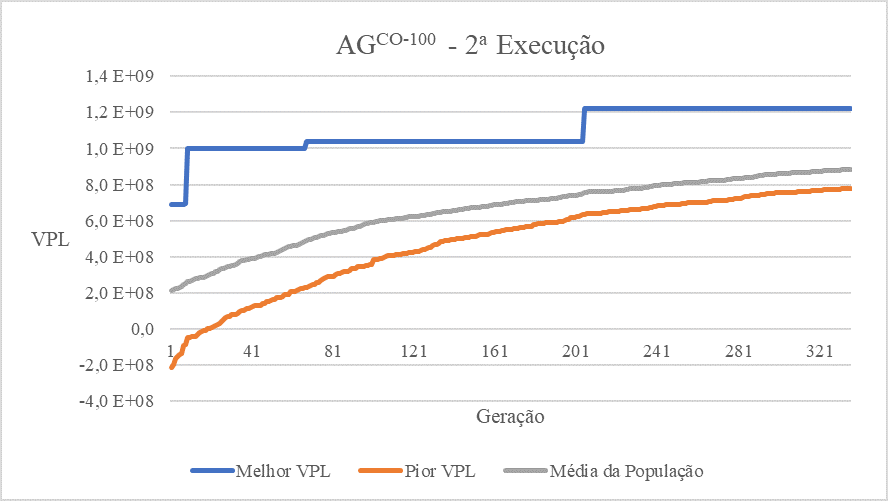
\includegraphics[scale=1]{apxD/2}
\caption{Evolução do VPL para a segunda execução da primeira versão modificada de Algoritmo de Regime Permanente.}
\label{fig:graphRPM-02}
\end{figure}

\begin{figure}[H]
\centering
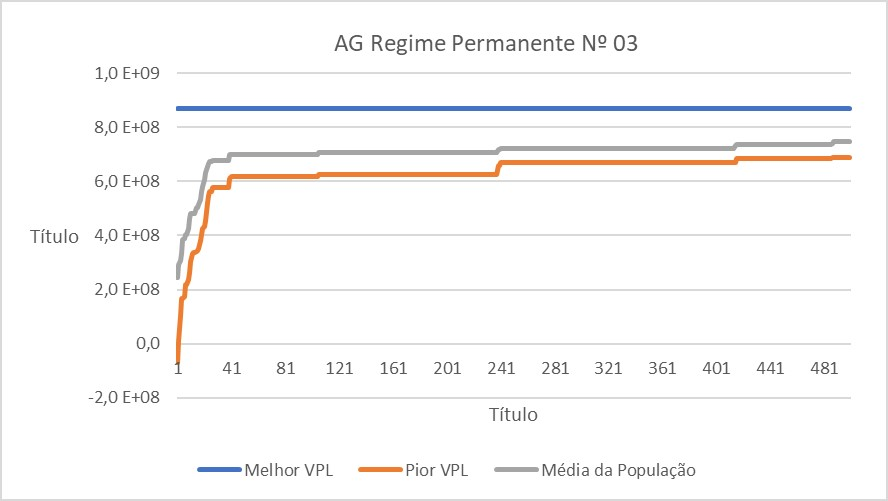
\includegraphics[scale=1]{apxD/3}
\caption{Evolução do VPL para a terceira execução da primeira versão modificada de Algoritmo de Regime Permanente.}
\label{fig:graphRPM-03}
\end{figure}

\begin{figure}[H]
\centering
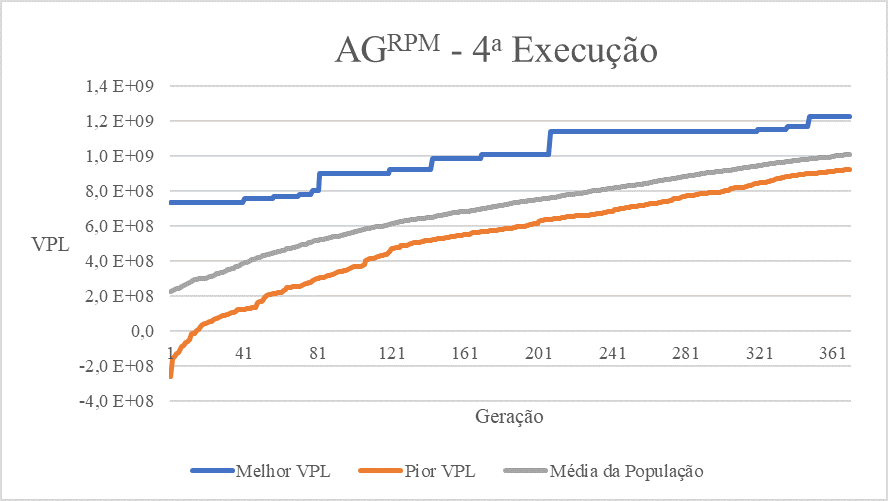
\includegraphics[scale=1]{apxD/4}
\caption{Evolução do VPL para a quarta execução da primeira versão modificada de Algoritmo de Regime Permanente.}
\label{fig:graphRPM-04}
\end{figure}

\begin{figure}[H]
\centering
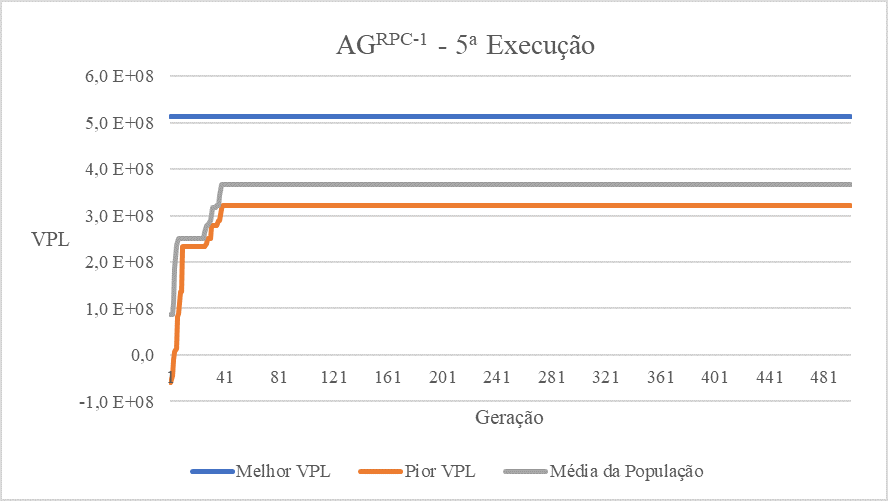
\includegraphics[scale=1]{apxD/5}
\caption{Evolução do VPL para a quinta execução da primeira versão modificada de Algoritmo de Regime Permanente.}
\label{fig:graphRPM-05}
\end{figure}

\begin{figure}[H]
\centering
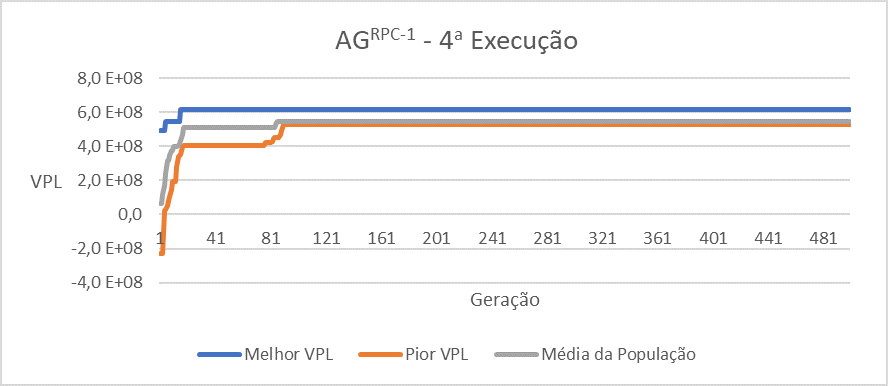
\includegraphics[scale=1]{apxD/6}
\caption{Evolução do VPL para a sexta execução da primeira versão modificada de Algoritmo de Regime Permanente.}
\label{fig:graphRPM-06}
\end{figure}

\begin{figure}[H]
\centering
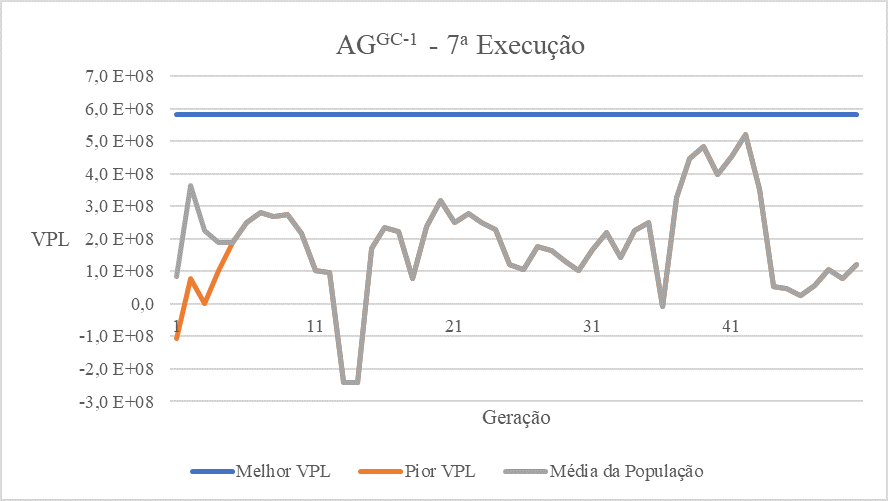
\includegraphics[scale=1]{apxD/7}
\caption{Evolução do VPL para a sétima execução da primeira versão modificada de Algoritmo de Regime Permanente.}
\label{fig:graphRPM-07}
\end{figure}

\begin{figure}[H]
\centering
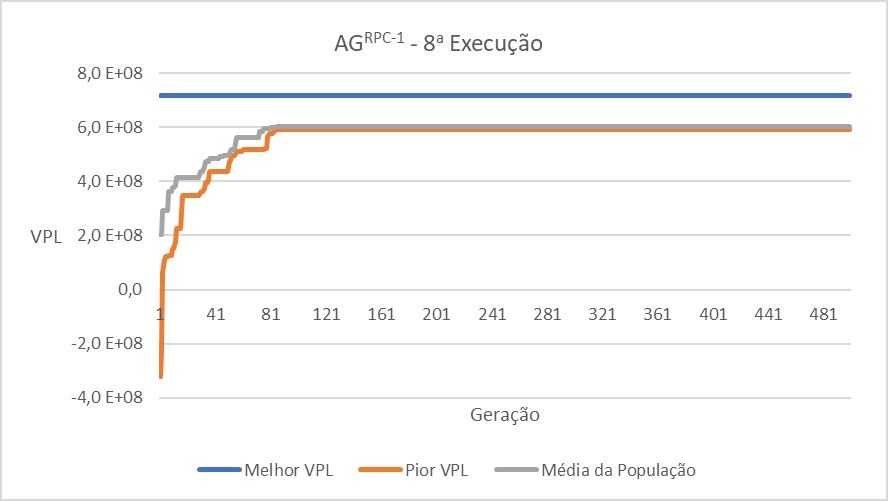
\includegraphics[scale=1]{apxD/8}
\caption{Evolução do VPL para a oitava execução da primeira versão modificada de Algoritmo de Regime Permanente.}
\label{fig:graphRPM-08}
\end{figure}

\begin{figure}[H]
\centering
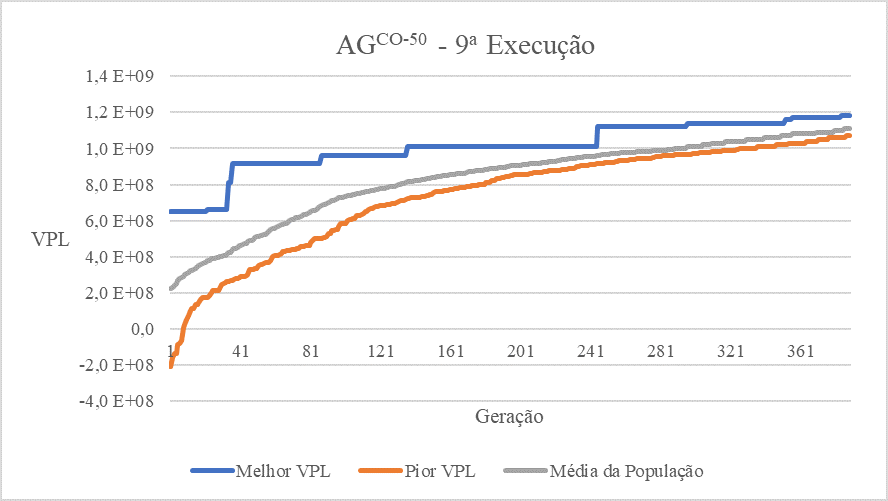
\includegraphics[scale=1]{apxD/9}
\caption{Evolução do VPL para a nona execução da primeira versão modificada de Algoritmo de Regime Permanente.}
\label{fig:graphRPM-09}
\end{figure}

\begin{figure}[H]
\centering
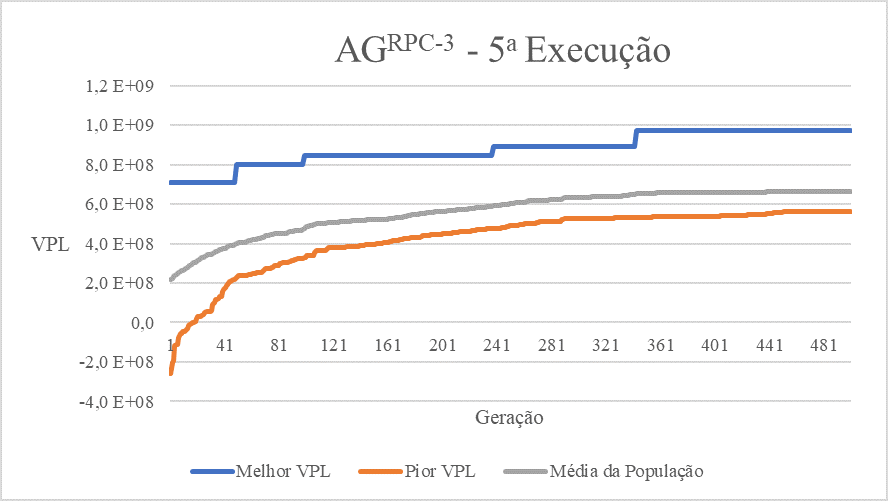
\includegraphics[scale=1]{apxD/10}
\caption{Evolução do VPL para a décima execução da primeira versão modificada de Algoritmo de Regime Permanente.}
\label{fig:graphRPM-10}
\end{figure}